\documentclass[a4paper,10pt]{memoir}
\usepackage[italian]{babel}
\usepackage{wrapfig}

% import package
\usepackage{FrontespizioSapienza}

\renewcommand\chapterheadstart{}
\renewcommand\printchaptername{}
\renewcommand\chapternamenum{}
\renewcommand\printchapternum{}
\renewcommand\afterchapternum{}
\renewcommand\printchaptertitle[1]{\chaptitlefont \thechapter. \space #1}

% declare info
\FSSTitolo{Ottimizzazione delle risorse nell'uso di servizi in background in SeismoCloud per Android}
\FSSFacolta{Facoltà di Ingegneria dell'Informazione, Informatica e Statistica}
\FSSCorso{Informatica}

\FSSCandidato{Enrico Bassetti}
\FSSMatricola{1401568}
\FSSRelatore{Emanuele Panizzi}
\FSSCorrelatore{}
\FSSAnnoAccademico{2016/2017}


\begin{document}
  
  
\frontmatter


% print title
\maketitle
\cleardoublepage

% rest of the document
\begin{abstract}
	\thispagestyle{plain}
	Sommario della tesi.
\end{abstract}
\cleardoublepage

\tableofcontents
\cleardoublepage

\mainmatter

%\setlength{\intextsep}{1pt}%

\chapter{Introduzione}

\section{I terremoti e la loro origine}


\begin{wrapfigure}{r}{0.30\textwidth}
\label{fig:litosfera}
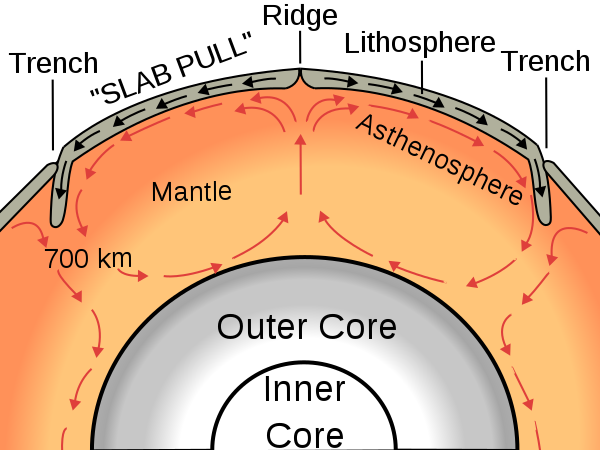
\includegraphics[width=0.30\textwidth]{introduzione/oceanic_spreading}
\end{wrapfigure}

La Terra è formata, nei primi 200 km di bordo esterno, da una zona chiamata \textit{litosfera}, di cui fa parte la \textit{crosta terrestre} con le terre emerse ed i fondali marini/oceanici. La \textit{litosfera} è divisa in parti, chiamate \textbf{placche tettoniche}, che "gallegiano" sul \textit{mantello superiore}. Queste placche sono continuamente spinte in direzioni diverse da \textit{moti convettivi} generati dalla temperatura elevata del nucleo. La zona di confine di queste placche viene chiamata \textbf{faglia}, e presenta diverse caratteristiche a seconda delle direzioni delle placche: se due placche si avvicinano, una delle due placche verrà immersa nel mantello sotto l'altra (\textit{subduzione}); se due placche si allontanano, una nuova parte della litosfera viene generata dalla roccia fusa proveniente dal mantello; infine, se due placche si muovo nella stessa direzione ma in senso opposto, siamo in presenza di \textit{margini di scorrimento}.

\begin{wrapfigure}[12]{r}{0.30\textwidth}
\label{fig:mappafaglie}
\caption{Mappa delle faglie italiane attive}
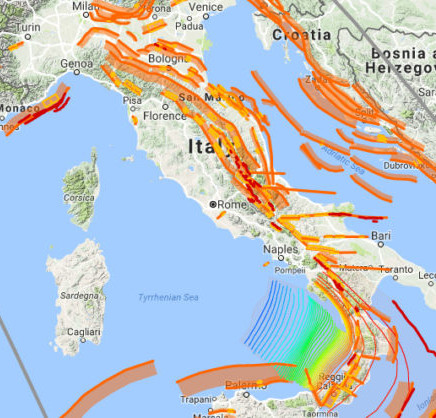
\includegraphics[width=0.30\textwidth]{introduzione/mappa_faglie_italiane2}
\end{wrapfigure}

Il movimento delle placche nei margini, tuttavia, non è libero da attrito: a seconda del materiale, della profondità e della conformazione della roccia presente nella faglia, la faglia stessa tende ad \textbf{opporsi} al movimento delle placche, accumulando energia da attrito, la quale viene rilasciata repentinamente (al superamento della massima forza d'attrito) come energia meccanica (le cosiddette \textit{onde sismiche}) generando un \textit{terremoto} (o sisma).

\section{Analisi e misura dei terremoti}

Per misurare l'energia sprigionata da un evento sismico, individuare il punto di origine (epicentro/ipocentro) e altre caratteristiche, si utilizzano i \textbf{sismometri}, ovvero apparati dotati di accelerometri molto precisi, filtri e amplificatori in grado di rilevare l'accelerazione sulle tre componenti (X-Y-Z) e produrre un \textit{sismogramma} (Figura \ref{fig:sismogramma}).

\begin{figure}[p]
\label{fig:retesensori}
\caption{La rete IV - Italian Seismic Network}
\centering
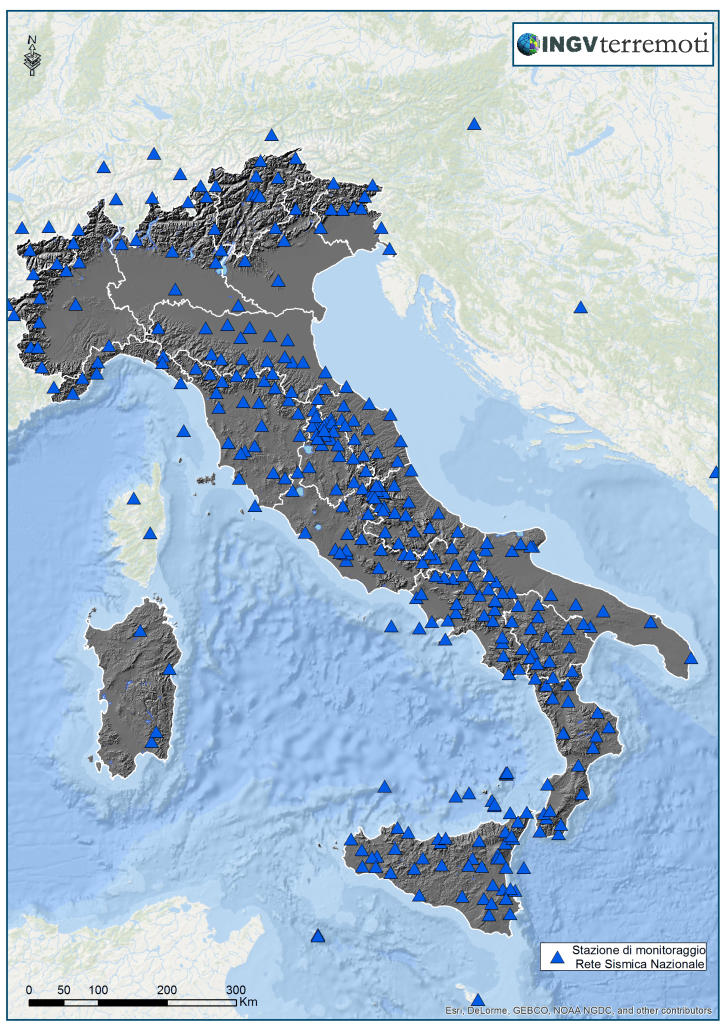
\includegraphics[width=10cm]{introduzione/rete_ingv}
\end{figure}

\begin{figure}[h]
\label{fig:sismogramma}
\caption{Esempio di sismogramma}
\centering
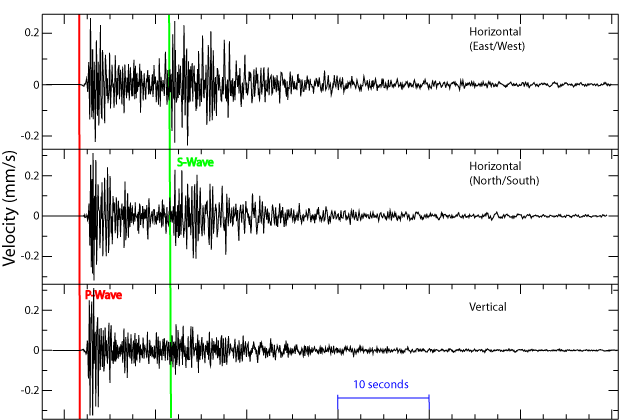
\includegraphics[width=10cm]{introduzione/seismogram}
\end{figure}

Attualmente nel mondo sono presenti diverse reti di rilevamento. Per l'Italia INGV riceve le informazioni da 27 reti sismiche (compresa la rete principale italiana \textit{IV - Italian Seismic Network}) per un totale di più di 800 sismometri (gran parte sul territorio nazionale, alcuni su paesi confinanti).

L'energia sprigionata viene misurata in \textbf{magnitudo} su una scala di valutazione chiamata \textbf{Richter}, mentre gli eventuali danni provocati vengono espressi in \textit{intensità del terremoto} tramite valori della scala \textbf{Mercalli-Cancani-Sieberg}, o MCS \footnote{Le due scale non hanno un legame diretto: un terremoto di piccola magnitudo può fare molti danni in alcune situazioni (e quindi essere di elevata intensità MCS); viceversa un terremoto di magnitudo molto elevata può avere intensità molto bassa in altre situazioni.}.

Infine possiamo distinguere il punto di origine del terremoto sotto la superficie, chiamato \textbf{epicentro}, e la proiezione di questo punto sulla superficie terrestre, chiamato \textbf{ipocentro} \footnote{Stein, Seth; Wysession, Michael (2009). An Introduction to Seismology, Earthquakes, and Earth Structure. John Wiley \& Sons. ISBN 978-1444311310}.

\begin{figure}[h]
\label{fig:epiipo}
\caption{Epicentro, ipocentro (o focus) e faglia (\textit{fault plane})}
\centering
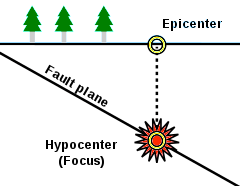
\includegraphics[scale=0.5]{introduzione/epicenter_diagram}
\end{figure}


\section{Prevedere o arginare i terremoti}

L'Italia è sottoposta, ogni giorno, ad un numero di terremoti nell'ordine del \textbf{centinaio di scosse}\footnote{Dati provenienti dal Centro Nazionale Terremoti: http://cnt.rm.ingv.it/}. Quasi tutti questi sismi sono classificati come \textit{microterremoti} (di magnitudo $<$ 2), poiché sono talmente deboli da essere percepibili solo dagli strumenti. Tuttavia, essendo l'Italia zona di confine tra la placca Europea e la placca Africana (con quest'ultima che si muove verso il Nord), la quantità di energia accumulata dalle faglie può generare terremoti in grado di infliggere ingenti danni.

Come in tutte le calamità naturali (e non), abbiamo diversi ambiti da considerare:
\begin{itemize}
\item la \textbf{prevenzione}, ovvero l'attuazione delle politiche in grado di minimizzare la probabilità che un evento accada e minimizzare il rischio all'accadere dell'evento
\item la \textbf{previsione}, ovvero l'utilizzo di tecniche e tecnologie che permettono di indicare \textit{quando un evento accadrà} (con una certa affidabilità)
\item la \textbf{gestione dell'emergenza} e del post-emergenza, ovvero delle azioni da mettere in capo durante e dopo il presentarsi di una calamità
\end{itemize}

Nella fattispecie dei terremoti, la \textbf{previsione} è tutt'ora materiale di studio da parte del mondo scientifico (ad esempio dal nostro \textbf{Istituto Nazionale di Geofisica e Vulcanologia}, o INGV) poiché risulta impossibile capire, allo stato attuale, quando e dove accadrà il prossimo sisma \footnote{Alessandro Amato (2016). Sotto i nostri piedi. Codice edizioni, Torino. ISBN 978-8875785727}. Nel tempo, tuttavia, i vari dati raccolti riguardo ai terremoti hanno permesso di costruire delle mappe di pericolosità sismica\footnote{Pubblicate per la prima volta nel 2004 e poi aggiornate man mano: http://zonesismiche.mi.ingv.it/}, le quali indicano zone con maggiore probabilità di terremoti importanti, andando ad integrare le azioni di informazione e di formazione che fanno parte della \textbf{prevenzione}.

\begin{wrapfigure}[12]{r}{0.25\textwidth}
\centering
\label{fig:timelinecom}
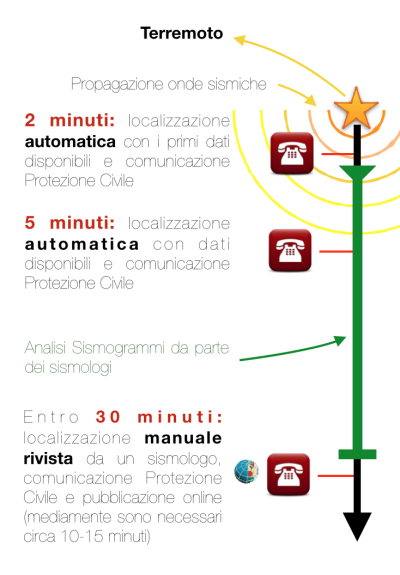
\includegraphics[width=0.25\textwidth]{introduzione/tempi_comunicazioni}
\end{wrapfigure}

Nella gestione dell'emergenza possiamo riportare quello che avviene allo stato attuale all'accadere di un terremoto, rilevato (per l'Italia) dalla rete di sismometri di INGV: nel momento in cui un sisma viene percepito da un numero congruo di stazioni di rilevamento, il sistema effettua verifiche e calcoli e, \textbf{entro due minuti}, è in grado di fornire una prima stima della magnitudo, dell'epicentro e della profondità (dati che poi vengono comunicati alla Protezione Civile). Successivamente, \textbf{entro 5 minuti} dal sisma, tutte le stazioni di rilevamento sono utilizzate per individuare le caratteristiche del terremoto in modo più preciso. Infine, \textbf{entro 30 minuti}, una verifica manuale da parte dei tecnici e ingegneri di INGV permette di avere il dato definitivo che viene di nuovo comunicato alla Protezione Civile e al pubblico \footnote{La pubblicazione avviene sul sito del Centro Nazionale Terremoti http://cnt.rm.ingv.it/ oppure tramite le pagine ufficiali sui principali Social Network}.

\section{Il progetto SeismoCloud}

Il progetto SeismoCloud nasce dalla collaborazione dall'\textbf{Università degli Studi di Roma "La Sapienza"} e l'\textbf{Istituto Nazionale di Geofisica e Vulcanologia}. L'obiettivo di questo progetto è quello di implementare un sistema di \textbf{early warning} in \textit{crowdsourcing}\footnote{Un sistema si dice in \textit{crowdsourcing} quando i dati per il suo funzionamento vengono forniti dagli stessi utenti} per i terremoti, in grado di inserirsi nel \textit{gap} presente dal momento in cui il terremoto accade, al momento in cui INGV è in grado di individuarlo. Lo scopo del sistema quindi è di individuare i terremoti \textit{in tempo reale}, ovvero alla loro apparizione nell'ipocentro, ed \textbf{anticipare} l'onda sismica (che viaggia, mediamente, ad una velocità di 5 km/s) avvertendo la popolazione nel raggio di azione del terremoto.
Essendo un sistema in \textit{crowdsourcing}, i dati della rete provengono dagli utenti; sono disponibili applicazioni per smartphones (Android, iOS) e dispositivi \textit{Internet of Things} (Arduino, NodeMCU, Raspberry PI) in grado di collezionare, con apposito sensore, i dati di accelerazione nei tre assi (X, Y, e Z). Data la poca precisione di questi sensori in relazione ai sensori della Rete Sismica Nazionale, il sistema di valutazione di SeismoCloud prende in considerazione la quantità di rilevazioni.

\pagebreak

\section{Architettura del sistema}

(inserire qui un grafico dell'architettura del sistema)

\section{Algoritmo di rilevamento}

Il funzionamento del sistema è il seguente: ogni dispositivo (smartphone o dispositivo \textit{IoT}) ha almeno due stati: \textbf{IDLE} e \textbf{QUAKE}. Un dispositivo nello stato di \textbf{IDLE} effettua una rilevazione dell'accelerazione su ogni asse ogni $50ms$, e viene calcolata la componente del vettore risultante mediante la formula~\ref{eq:vettoreris}. Il valore viene quindi confrontato con un valore di soglia calcolato (\ref{eq:soglia}) in modo da filtrare il rumore di fondo e, se la rilevazione risulta superiore alla soglia, il dispositivo informa il server comunicando l'attuale accelerazione rilevata ed il momento della rilevazione espresso in tempo UNIX\footnote{Il "tempo UNIX" è definito come il numero di secondi dallo \textit{UNIX Epoch Time}, ovvero dal 1 Gennaio 1970} (con precisione di $\pm1ms$), e successivamene passa allo stato di \textbf{QUAKE}.

\begin{equation} \label{eq:vettoreris}
Acceleration = \sqrt{Value(X)^2 + Value(Y)^2 + Value(Z)^2}
\end{equation}

Per ogni valore rilevato nello stato \textit{IDLE}, inoltre, vengono aggiornati i seguenti valori:
\begin{equation}
\Delta = Acceleration - \rho
\end{equation}
\begin{equation}
\rho = \rho + {\Delta \over |detections|}
\end{equation}
\begin{equation}
\sigma = \sigma + \Delta * (Acceleration - \rho)
\end{equation}
\begin{equation} \label{eq:soglia}
Threshold = \rho + (\sqrt{\sigma \over (|detections|-1)} * \alpha)
\end{equation}

dove: \begin{itemize}
\item $Acceleration \in Z^+$ rappresenta il valore di accelerazione attuale
\item $\rho \in Z^+$ è la media dei valori delle rilevazioni, calcolata mediante un \textit{algoritmo online}\footnote{Un algoritmo viene definito \textit{online} se è in grado di processare un oggetto di input per volta (mantenendo l'invariante che il risultato rappresenta il valore atteso), potenzialmente per un numero infinito di oggetti}
\item $\sigma \in Z^+$ rappresenta lo scarto quadratico medio
\item $Threshold \in Z^+$ rappresenta la soglia di confronto per il valore di accelerazione, utilizzata per decidere se è da informare il server
\item $\alpha \in Z^+$ rappresenta un valore moltiplicativo fornito dal server (aggiornato a seguito, ad esempio, di eccessive segnalazioni o soglia troppo alta)
\end{itemize}


\chapter{Ottimizzazione energetica: i contesti di attivazione}

Qui si parla delle politiche di spegnimento (con algoritmo di backoff) in caso di posizione non utile o mancanza di dati utili al rilevamento (prima posizione, rilevato movimento localizzazione) o stato batteria/connessione.

\chapter{Ottimizzazione energetica: i sensori}

Si spiega anche l'attivazione programmata del magnetometro dopo l'attività dell'accelerometro, inizialmente pensata per risparmiare CPU ed energia, e come questo meccanismo sia stato dismesso poiché effettivamente non comportava nessun risparmio energetico (il sistema mag+accel è sempre attivo).

\chapter{Ottimizzazione energetica: la curva di scarica}

Qui parlo dell'algoritmo che segue la curva di scarica. Tips: mostrare i dati provenienti dal database con interrogazioni statistiche

\chapter{Ottimizzazione del processore: la comunicazione con il front-end}

Qui si descrive la politica utilizzata per mantere l'applicazione attiva (notifica permanente) poiché Android pone le applicazioni in sleep. Si spiega anche il wakelock sulla CPU, la sospensione dell'aggiornamento dati in background delle activity quando non sono in vista.

\chapter{Ottimizzazione della rete: MQTT}

Si spiega come l'introduzione dell'MQTT abbia ridotto il carico sulla rete per lo scambio dati con il server.

\chapter{Ottimizzazione della rete: Pushback}

Parlare del meccanismo di Pushback per l'invio dei dati (ad esempio survey) in background in modo ottimizzato in caso di problemi di rete (invio asincrono).

\chapter{Ottimizzazione dell'uso di memoria nel codice}

Qui si descrive la politica utilizzata, nella costruzione del codice, per minimizzare lo spreco di memoria (esempio: media/varianza mobile).

%
%\chapter{Sviluppo e test}
%
%Si spiega l'adozione di particolari meccanismi per la gestione ottimizzata del processo di sviluppo:
%
%\begin{itemize}
%\item Utilizzo della libreria ACRA per l'immediata segnalazione di errori della app (da produzione)
%\item Utilizzo della libreria LeakCanary per la ricerca di memory leak
%\item Utilizzo delle librerie Parceler e Android Annotations per ridurre la quantità di codice ridondante
%\item Sistemi di controllo versione: branch per funzionalità, sviluppo parallelo
%\item Continuos integration per la verifica dei build ed instrumentation test
%\item Verifica del codice tramite SonarQube per aderenza agli standard Java/Android e risultati di analisi statica del codice
%\end{itemize}

\chapter{Sviluppi futuri}

\begin{itemize}
\item Utilizzo di un sistema di spegnimento controllato dal server per l'ottimizzazione geografica
\item Utilizzo di sensori dedicati (es. Samsung Significant Motion Sensor) per il wake-up
\item Riscrittura parti critiche in codice nativo per l'esecuzione ottimizzata e rapida (con conseguente aumento del periodo di idle del telefono)
\end{itemize}

\end{document}
